El filtro colorizar modifica cada pixel de una imagen color de acuerdo a una ecuación que depende
de los máximos valores de los canales R, G y B entre los píxeles del cuadrado de lado 3 formado
por el pixel original y sus 8 vecinos inmediatos.

El problema principal a resolver es minimizar la cantidad de accesos a memoria y paralelizar lo más
posible las comparaciones necesarias para hallar el máximo valor de cada canal en el cuadrado
de lado 3 correspondiente a cada pixel.


%%%%%%%%%%%%%%%%%%%%%%%%%%%%%%%%%%%%%%%%%%%%%%%%%%%%%%%%%%%%%%%%%%%%%%%%%%%%%%%
%% Descripción del ciclo                                                     %%
%%%%%%%%%%%%%%%%%%%%%%%%%%%%%%%%%%%%%%%%%%%%%%%%%%%%%%%%%%%%%%%%%%%%%%%%%%%%%%%


\subsubsection{Descripción del ciclo}

Para cada pixel, dividimos el ciclo en cuatro etapas:

\begin{enumerate}
    \item \textbf{Lectura de píxeles vecinos:}
        Cargamos los píxeles de cada fila del cuadrado en \xmm{1}, \xmm{2} y \xmm{3}.
    \item \textbf{Búsqueda de máximos por canal:}
        Separamos cada pixel por canal, y comparamos sucesivamente los valores de cada canal
        entre sí para hallar los máximos.
    \item \textbf{Hallar $\Phi_{R,G,B}$:}
        Hallamos los valores de $\Phi_R$, $\Phi_G$ y $\Phi_B$ utilizando los máximos
        obtenidos en la etapa anterior.
    \item \textbf{Escritura de pixel destino:}
        Computamos el valor del pixel destino y lo escribimos en la imagen.
\end{enumerate}

Veamos a continuación cada etapa en detalle.


%%%%%%%%%%%%%%%%%%%%%%%%%%%%%%%%%%%%%%%%%%%%%%%%%%%%%%%%%%%%%%%%%%%%%%%%%%%%%%%
%% Lectura de píxeles                                                        %%
%%%%%%%%%%%%%%%%%%%%%%%%%%%%%%%%%%%%%%%%%%%%%%%%%%%%%%%%%%%%%%%%%%%%%%%%%%%%%%%


\subsubsection{Lectura de píxeles vecinos}

Cargamos los píxeles de cada fila del cuadrado de lado 3 como se indica a continuación:

\begin{pseudocodigo}
    \STATE \texttt{MOVDQU} \xmm{1}, $src[y-1][x-3]$
    \STATE \texttt{MOVDQU} \xmm{2}, $src[y][x-3]$
    \STATE \texttt{MOVDQU} \xmm{3}, $src[y+1][x-3]$        
\end{pseudocodigo}

Contenido de los registros \xmm{1}, \xmm{2} y \xmm{3} en este instante:

\begin{center}
    \begin{tikzpicture}[scale=0.75]
        \registroDieciseis{}{0}{0}
                          {$\ast$}{$\ast$}{$\ast$}{$\ast$}{$\ast$}{$\ast$}{$\ast$}
                          {$R$}{$G$}{$B$}{$R$}{$G$}{$B$}{$R$}{$G$}{$B$}
    \end{tikzpicture}
\end{center}

El símbolo $\ast$ representa información de píxeles adyacentes que no nos interesa.

En el caso de estar leyendo los últimos píxeles de la última fila, las lecturas
se realizan desplazándonos hacia atrás sobre el eje X tantos píxeles como sea
necesario, de forma tal que la parte alta de cada registro XMM esté alineada
con el último pixel. En este caso el contenido de cada registro sería
el siguiente:

\begin{center}
    \begin{tikzpicture}[scale=0.75]
        \registroDieciseis{}{0}{0}
                          {$R$}{$G$}{$B$}{$R$}{$G$}{$B$}{$R$}{$G$}{$B$}
                          {$\ast$}{$\ast$}{$\ast$}{$\ast$}{$\ast$}{$\ast$}{$\ast$}
    \end{tikzpicture}
\end{center}

Luego de realizar esta lectura, reacomodamos los bytes con \texttt{PSHUFB}
para tenerlos en el mismo orden que en el caso normal, y procedemos normalmente.

%%%%%%%%%%%%%%%%%%%%%%%%%%%%%%%%%%%%%%%%%%%%%%%%%%%%%%%%%%%%%%%%%%%%%%%%%%%%%%%
%% Búsqueda de máximos                                                       %%
%%%%%%%%%%%%%%%%%%%%%%%%%%%%%%%%%%%%%%%%%%%%%%%%%%%%%%%%%%%%%%%%%%%%%%%%%%%%%%%


\subsubsection{Búsqueda de máximos por canal}

El siguiente paso es comparar los valores de cada canal entre sí para hallar los máximos.

Lo primero que hacemos es reordenar los bytes en \xmm{1}, \xmm{2} y \xmm{3}:

\begin{pseudocodigo}
    \STATE \texttt{PSHUFB} \xmm{1}, \textit{máscara}
    \STATE \texttt{PSHUFB} \xmm{2}, \textit{máscara}
    \STATE \texttt{PSHUFB} \xmm{3}, \textit{máscara}
\end{pseudocodigo}

La \textit{máscara} provista es tal que los bytes de los registros quedan
reordeados de la siguiente forma:

\begin{center}
    \begin{tikzpicture}[scale=0.75]
        \registroDieciseis{}{0}{0}
                          {0}{0}{0}{0}
                          {0}{$R$}{$R$}{$R$}
                          {0}{$G$}{$G$}{$G$}
                          {0}{$B$}{$B$}{$B$}
    \end{tikzpicture}
\end{center}

A continuación, buscamos los máximos byte a byte entre \xmm{1} y \xmm{2} y luego entre
\xmm{1} y \xmm{3} de manera de obtener los máximos por canal ``columna a columna'':

\begin{pseudocodigo}
    \STATE \texttt{PMAXUB} \xmm{1}, \xmm{2}
    \STATE \texttt{PMAXUB} \xmm{1}, \xmm{3}    
\end{pseudocodigo}

La siguiente ilustración muestra lo que ocurre con los primeros 3 bytes de
\xmm{1}, \xmm{2} y \xmm{3}, que contienen los valores del canal B para los
tres píxeles de las filas 1, 2 y 3 respectivamente:

\begin{center}
    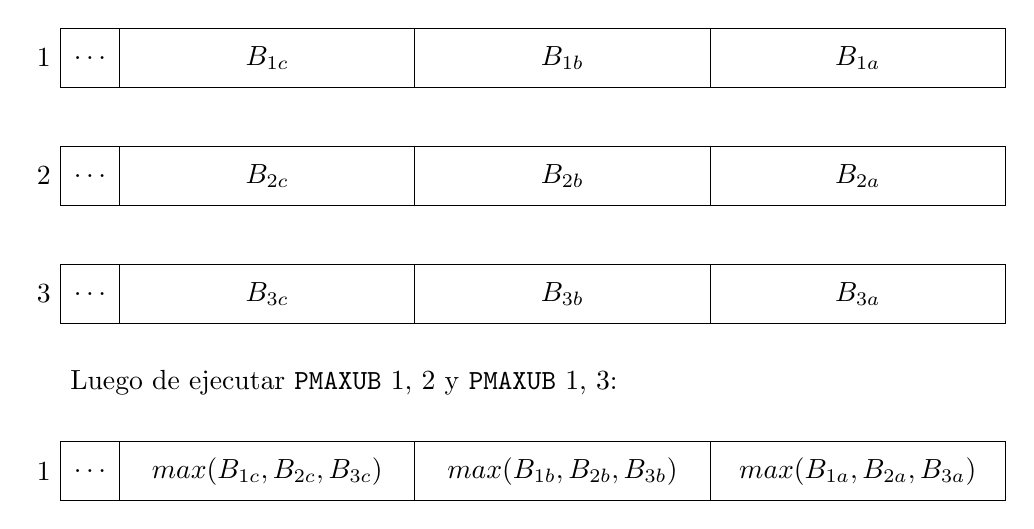
\begin{tikzpicture}[scale=0.75]
        \foreach \i in {1, ..., 3}
        {
            \draw (0,  {-(\i - 1) * 2 + 0.5}) node[anchor=east]{\xmm{\i}};
            \draw (0,  {-(\i - 1) * 2}) rectangle +(1, 1) +(0.5, 0.5) node{$\dots$};
            \draw (1,  {-(\i - 1) * 2}) rectangle +(5, 1) +(2.5, 0.5) node{$B_{{\i}c}$};
            \draw (6,  {-(\i - 1) * 2}) rectangle +(5, 1) +(2.5, 0.5) node{$B_{{\i}b}$};        
            \draw (11, {-(\i - 1) * 2}) rectangle +(5, 1) +(2.5, 0.5) node{$B_{{\i}a}$};
        }

        \draw (0, -5) node[anchor=west]
            {Luego de ejecutar \texttt{PMAXUB} \xmm{1}, \xmm{2} y
                               \texttt{PMAXUB} \xmm{1}, \xmm{3}:};

        \draw (0, {-7 + 0.5}) node[anchor=east]{\xmm{1}};
        \draw (0,  -7) rectangle +(1, 1) +(0.5, 0.5) node{$\dots$};
        \draw (1,  -7) rectangle +(5, 1) +(2.5, 0.5) node{$max(B_{1c}, B_{2c}, B_{3c})$};
        \draw (6,  -7) rectangle +(5, 1) +(2.5, 0.5) node{$max(B_{1b}, B_{2b}, B_{3b})$};        
        \draw (11, -7) rectangle +(5, 1) +(2.5, 0.5) node{$max(B_{1a}, B_{2a}, B_{3a})$};        
    \end{tikzpicture}
\end{center}

Lo mismo ocurre con el resto de los bytes que contienen los valores para los canales R y G.

En este instante el contenido de \xmm{1} es el siguiente:

\begin{center}
    \begin{tikzpicture}[scale=0.75]
        \registroDieciseis{\xmm{1}}{0}{0}
                          {0}{0}{0}{0}
                          {0}{$R_c$}{$R_b$}{$R_a$}
                          {0}{$G_c$}{$G_b$}{$G_a$}
                          {0}{$B_c$}{$B_b$}{$B_a$}
    \end{tikzpicture}
\end{center}

Donde $B_a = max(B_{1a}, B_{2a}, B_{3a})$, $\dots$, $R_c = max(R_{1c}, R_{2c}, R_{3c})$.

Para encontrar $max_R$, $max_G$ y $max_B$ aún nos falta maximizar las tuplas
$(R_a, R_b, R_c)$, $(G_a, G_b, G_c)$ y $(B_a, B_b, B_c)$.

Extraemos las tres triplas $(R, G, B)$ del registro \xmm{1} usando
\texttt{PSHUFB} con las máscaras correspondientes y las almacenamos por separado en
\xmm{1}, \xmm{2} y \xmm{3}, de manera de tener un único valor R, G y B en cada uno de
estos registros, para poder buscar los máximos en paralelo columna a columna con
\texttt{PMAXUB}, como hicimos antes.

Gráficamente, podemos representar esta serie de pasos de la siguiente manera:

\begin{center}
    \begin{tikzpicture}[scale=0.75, >=stealth]
        \registroDieciseis{\xmm{1}}{0}{10}
                          {0}{0}{0}{0}
                          {0}{$R_c$}{$R_b$}{$R_a$}
                          {0}{$G_c$}{$G_b$}{$G_a$}
                          {0}{$B_c$}{$B_b$}{$B_a$}

        \draw [->, thick] (15.5, 10) -- (15.5, 8); % Ba
        \draw [->, thick] (14.5, 10) -- (15.5, 6); % Bb
        \draw [->, thick] (13.5, 10) -- (15.5, 4); % Bc

        \draw [->, thick] (11.5, 10) -- (11.5, 8); % Ga
        \draw [->, thick] (10.5, 10) -- (11.5, 6); % Gb
        \draw [->, thick]  (9.5, 10) -- (11.5, 4); % Gc

        \draw [->, thick]  (7.5, 10) --  (7.5, 8); % Ra
        \draw [->, thick]  (6.5, 10) --  (7.5, 6); % Rb
        \draw [->, thick]  (5.5, 10) --  (7.5, 4); % Rc        

        \draw (0, 9) node[anchor=west, fill=white]{Luego de extraer las triplas:};

        \registroDieciseis{\xmm{1}}{0}{7}
                          {0}{0}{0}{0}
                          {0}{0}{0}{$R_a$}
                          {0}{0}{0}{$G_a$}
                          {0}{0}{0}{$B_a$}

        \registroDieciseis{\xmm{2}}{0}{5}
                          {0}{0}{0}{0}
                          {0}{0}{0}{$R_b$}
                          {0}{0}{0}{$G_b$}
                          {0}{0}{0}{$B_b$}

        \registroDieciseis{\xmm{3}}{0}{3}
                          {0}{0}{0}{0}
                          {0}{0}{0}{$R_c$}
                          {0}{0}{0}{$G_c$}
                          {0}{0}{0}{$B_c$}

        \draw (0, 2) node[anchor=west]
            {Luego de ejecutar \texttt{PMAXUB} \xmm{1}, \xmm{2} y
                               \texttt{PMAXUB} \xmm{1}, \xmm{3}:};

        \registroDieciseis{\xmm{1}}{0}{0}
                          {0}{0}{0}{0}
                          {0}{0}{0}{$R^\ast$}
                          {0}{0}{0}{$G^\ast$}
                          {0}{0}{0}{$B^\ast$}
    \end{tikzpicture}
\end{center}

Donde $R^\ast = max_R$, $G^\ast = max_G$ y $B^\ast = max_B$.

Finalmente extraemos los máximos con \texttt{PSHUFD} y \texttt{MOVD},
y los guardamos en registros de propósito general, para usarlos en la
siguiente etapa.


%%%%%%%%%%%%%%%%%%%%%%%%%%%%%%%%%%%%%%%%%%%%%%%%%%%%%%%%%%%%%%%%%%%%%%%%%%%%%%%
%% Hallar Phi                                                               %%
%%%%%%%%%%%%%%%%%%%%%%%%%%%%%%%%%%%%%%%%%%%%%%%%%%%%%%%%%%%%%%%%%%%%%%%%%%%%%%%


\subsubsection{Hallar $\Phi_{R,G,B}$}

Procedemos a computar $\Phi_R$, $\Phi_G$ y $\Phi_B$ de forma secuencial,
luego empaquetamos en \xmm{1} los valores hallados como se indica a continuación:

\begin{center}
    \begin{tikzpicture}[scale=0.75]
        \registroCuatro{\xmm{1}}{0}{0}{$\ast$}{$\Phi_R$}{$\Phi_G$}{$\Phi_B$}
    \end{tikzpicture}
\end{center}

Empaquetamos $\Phi_{R,G,B}$ de esta manera para facilitar las
comparaciones que realizaremos en la siguiente y última etapa.


%%%%%%%%%%%%%%%%%%%%%%%%%%%%%%%%%%%%%%%%%%%%%%%%%%%%%%%%%%%%%%%%%%%%%%%%%%%%%%%
%% Pixel destino                                                             %%
%%%%%%%%%%%%%%%%%%%%%%%%%%%%%%%%%%%%%%%%%%%%%%%%%%%%%%%%%%%%%%%%%%%%%%%%%%%%%%%


\subsubsection{Escritura de pixel destino}

Antes de escribir el pixel destino, debemos hallar el valor de cada canal.
Recordemos las ecuaciones:

\begin{center}
    $I_{dst_R}(i, j) = min(255, \Phi_R \ast I_{src_R}(i, j))$ \\
    $I_{dst_G}(i, j) = min(255, \Phi_G \ast I_{src_G}(i, j))$ \\
    $I_{dst_B}(i, j) = min(255, \Phi_B \ast I_{src_B}(i, j))$
\end{center}

Procedemos a hallar $I_{src_{R,G,B}}(i, j)$:

\begin{pseudocodigo}
    \STATE \texttt{MOVDQU} \xmm{2},   $src[j][i]$      \COMMENT{leo el pixel original}
    \STATE \texttt{PSHUFB} \xmm{2},   \textit{máscara} \COMMENT{reacomodo y limpio registro}
    \STATE \texttt{CVTDQ2PS} \xmm{2}, xmm{2}           \COMMENT{convierto cada canal a float}
\end{pseudocodigo}

En este instante \xmm{2} contiene el valor de cada canal del pixel original
convertido a punto flotante como se ilustra a continuación:

\begin{center}
    \begin{tikzpicture}[scale=0.75]
        \registroCuatro{\xmm{2}}{0}{0}{$\ast$}{$I_{src_R}$}{$I_{src_G}$}{$I_{src_B}$}
    \end{tikzpicture}
\end{center}

Multiplicamos cada canal por el valor $\Phi$ correspondiente y buscamos
el mínimo entre este producto y 255:

\begin{pseudocodigo}
    \STATE \texttt{MULPS}    \xmm{2}, \xmm{1} \COMMENT{\xmm{2} $\leftarrow$ $\Phi \ast I_{src}$}
    \STATE \texttt{MOVDQU}   \xmm{1}, \textit{tupla 255}
        \COMMENT{cargo el valor 255 en los 3 floats más bajos de \xmm{1}}
    \STATE \texttt{MINPS}    \xmm{1}, \xmm{2}
        \COMMENT{\xmm{1} $\leftarrow$ $min(255, \Phi \ast I_{src}) = I_{dst}$}
    \STATE \texttt{CVTPS2DQ} \xmm{1}, \xmm{1} \COMMENT{convertimos a enteros los $I_{dst}$ hallados}
\end{pseudocodigo}

El contenido de de \xmm{1} es ahora:

\begin{center}
    \begin{tikzpicture}[scale=0.75]
        \registroCuatro{\xmm{1}}{0}{0}{$\ast$}{$I_{dst_R}$}{$I_{dst_G}$}{$I_{dst_B}$}
    \end{tikzpicture}
\end{center}

Si bien los valores $I_{dst_{R,G,B}}$ resultantes de la conversión de punto flotante a
entero sin signo son de 32 bits, recordemos que nunca se exceden de 255, por lo que podemos
asumir que nuestro dato está en el byte más bajo de cada entero, mientras que en los bytes
restantes hay ceros. Entonces el contenido de \xmm{1} es:

\begin{center}
    \begin{tikzpicture}[scale=0.75]
        \registroDieciseis{\xmm{1}}{0}{0}
                          {$\ast$}{$\ast$}{$\ast$}{$\ast$}
                          {0}{0}{0}{$I_{dst_R}$}
                          {0}{0}{0}{$I_{dst_G}$}
                          {0}{0}{0}{$I_{dst_B}$}
    \end{tikzpicture}
\end{center}

Reordenamos los bytes con \texttt{PSHUFB}:

\begin{center}
    \begin{tikzpicture}[scale=0.75]
        \registroDieciseis{\xmm{1}}{0}{0}
                          {$\ast$}{$\ast$}{$\ast$}{$\ast$}
                          {0}{0}{0}{0}{0}{0}{0}{0}
                          {0}{$I_{dst_R}$}{$I_{dst_G}$}{$I_{dst_B}$}
    \end{tikzpicture}
\end{center}

Para terminar, extraemos $I_{dst_R}$, $I_{dst_G}$ y $I_{dst_B}$ con \texttt{MOVD}
y escribimos el pixel obtenido en la imagen destino.


%%%%%%%%%%%%%%%%%%%%%%%%%%%%%%%%%%%%%%%%%%%%%%%%%%%%%%%%%%%%%%%%%%%%%%%%%%%%%%%
%% Descripción del ciclo                                                     %%
%%%%%%%%%%%%%%%%%%%%%%%%%%%%%%%%%%%%%%%%%%%%%%%%%%%%%%%%%%%%%%%%%%%%%%%%%%%%%%%


\subsubsection{Comparación con la implementación C}

Escencialmente, la versión C de este filtro realiza la misma secuencia de operaciones,
pero accediendo a memoria de a un byte por vez, y realizando las comparaciones
sin paralelismo. Esto significa que se realizan:

\begin{itemize}
    \item $9 * 3 = 27$ accesos a memoria para obtener cada canal de los píxeles vecinos,
    \item 3 accesos a memoria para leer el pixel original,
    \item 3 accesos a memoria para escribir el pixel destino, y
    \item 24 comparaciones para hallar $max_{R,G,B}$.
\end{itemize}

Esto es un total de 33 accesos a memoria y 24 comparaciones.

En contraste, la implementación assembler realiza:

\begin{itemize}
    \item 3 accesos a memoria para obtener los píxeles vecinos,
    \item 1 acceso a memoria para leer el pixel original,
    \item 1 acceso a memoria para escribir el pixel destino, y
    \item 6 comparaciones para hallar $max_{R,G,B}$.
\end{itemize}

Es decir, un total de 5 accesos a memoria y 6 comparaciones.

Expresado de forma relativa, la implementación assembler realiza
el $15.2\%$ de accesos a memoria y el $25\%$ de comparaciones que su
contraparte en lenguaje C.


%%%%%%%%%%%%%%%%%%%%%%%%%%%%%%%%%%%%%%%%%%%%%%%%%%%%%%%%%%%%%%%%%%%%%%%%%%%%%%%
%% Rendimiento                                                               %%
%%%%%%%%%%%%%%%%%%%%%%%%%%%%%%%%%%%%%%%%%%%%%%%%%%%%%%%%%%%%%%%%%%%%%%%%%%%%%%%


\subsubsection{Rendimiento}

Observamos las siguientes cantidades de ciclos y ticks de reloj al realizar 100 iteraciones de ambas implementaciones con una imagen cuadrada de lado 512 y parámetro $\alpha = 0.5$:

\begin{center}
    \begin{tabular}{|l|l|l|l|}
        \hline
        Medición & Implementación C & Implementación assembler & Relación \\
        \hline
        Ticks    & 53062000890      & 1213052436               & $2.28\%$ \\
        Ciclos   & 530620000        & 12130524                 & $2.28\%$ \\
        \hline
    \end{tabular}
\end{center}

En la sección anterior evaluamos las relaciones de accesos a memoria y comparaciones
entre ambas implementaciones. Sin realizar un mayor análisis, éstas nos sirven
para tener una idea intuitiva de las mejoras que podríamos esperar de haber optimizado
utilizando instrucciones SIMD. Sin embargo el rendimiento obtenido fue casi un orden
de magnitud superior.

Luego de analizar el código assembler generado por el compilador, identificamos una
gran cantidad de accesos a memoria adicionales, producidos por el uso de variables locales
almacenadas en la pila. Esto ocurre tanto en el ciclo principal como en varios auxiliares.
Atribuímos la diferencia de performance a estos accesos a memoria que no tuvimos en cuenta
en nuestro análisis inicial.